\documentclass[1p]{elsarticle_modified}
%\bibliographystyle{elsarticle-num}

%\usepackage[colorlinks]{hyperref}
%\usepackage{abbrmath_seonhwa} %\Abb, \Ascr, \Acal ,\Abf, \Afrak
\usepackage{amsfonts}
\usepackage{amssymb}
\usepackage{amsmath}
\usepackage{amsthm}
\usepackage{scalefnt}
\usepackage{amsbsy}
\usepackage{kotex}
\usepackage{caption}
\usepackage{subfig}
\usepackage{color}
\usepackage{graphicx}
\usepackage{xcolor} %% white, black, red, green, blue, cyan, magenta, yellow
\usepackage{float}
\usepackage{setspace}
\usepackage{hyperref}

\usepackage{tikz}
\usetikzlibrary{arrows}

\usepackage{multirow}
\usepackage{array} % fixed length table
\usepackage{hhline}

%%%%%%%%%%%%%%%%%%%%%
\makeatletter
\renewcommand*\env@matrix[1][\arraystretch]{%
	\edef\arraystretch{#1}%
	\hskip -\arraycolsep
	\let\@ifnextchar\new@ifnextchar
	\array{*\c@MaxMatrixCols c}}
\makeatother %https://tex.stackexchange.com/questions/14071/how-can-i-increase-the-line-spacing-in-a-matrix
%%%%%%%%%%%%%%%

\usepackage[normalem]{ulem}

\newcommand{\msout}[1]{\ifmmode\text{\sout{\ensuremath{#1}}}\else\sout{#1}\fi}
%SOURCE: \msout is \stkout macro in https://tex.stackexchange.com/questions/20609/strikeout-in-math-mode

\newcommand{\cancel}[1]{
	\ifmmode
	{\color{red}\msout{#1}}
	\else
	{\color{red}\sout{#1}}
	\fi
}

\newcommand{\add}[1]{
	{\color{blue}\uwave{#1}}
}

\newcommand{\replace}[2]{
	\ifmmode
	{\color{red}\msout{#1}}{\color{blue}\uwave{#2}}
	\else
	{\color{red}\sout{#1}}{\color{blue}\uwave{#2}}
	\fi
}

\newcommand{\Sol}{\mathcal{S}} %segment
\newcommand{\D}{D} %diagram
\newcommand{\A}{\mathcal{A}} %arc


%%%%%%%%%%%%%%%%%%%%%%%%%%%%%5 test

\def\sl{\operatorname{\textup{SL}}(2,\Cbb)}
\def\psl{\operatorname{\textup{PSL}}(2,\Cbb)}
\def\quan{\mkern 1mu \triangleright \mkern 1mu}

\theoremstyle{definition}
\newtheorem{thm}{Theorem}[section]
\newtheorem{prop}[thm]{Proposition}
\newtheorem{lem}[thm]{Lemma}
\newtheorem{ques}[thm]{Question}
\newtheorem{cor}[thm]{Corollary}
\newtheorem{defn}[thm]{Definition}
\newtheorem{exam}[thm]{Example}
\newtheorem{rmk}[thm]{Remark}
\newtheorem{alg}[thm]{Algorithm}

\newcommand{\I}{\sqrt{-1}}
\begin{document}

%\begin{frontmatter}
%
%\title{Boundary parabolic representations of knots up to 8 crossings}
%
%%% Group authors per affiliation:
%\author{Yunhi Cho} 
%\address{Department of Mathematics, University of Seoul, Seoul, Korea}
%\ead{yhcho@uos.ac.kr}
%
%
%\author{Seonhwa Kim} %\fnref{s_kim}}
%\address{Center for Geometry and Physics, Institute for Basic Science, Pohang, 37673, Korea}
%\ead{ryeona17@ibs.re.kr}
%
%\author{Hyuk Kim}
%\address{Department of Mathematical Sciences, Seoul National University, Seoul 08826, Korea}
%\ead{hyukkim@snu.ac.kr}
%
%\author{Seokbeom Yoon}
%\address{Department of Mathematical Sciences, Seoul National University, Seoul, 08826,  Korea}
%\ead{sbyoon15@snu.ac.kr}
%
%\begin{abstract}
%We find all boundary parabolic representation of knots up to 8 crossings.
%
%\end{abstract}
%\begin{keyword}
%    \MSC[2010] 57M25 
%\end{keyword}
%
%\end{frontmatter}

%\linenumbers
%\tableofcontents
%
\newcommand\colored[1]{\textcolor{white}{\rule[-0.35ex]{0.8em}{1.4ex}}\kern-0.8em\color{red} #1}%
%\newcommand\colored[1]{\textcolor{white}{ #1}\kern-2.17ex	\textcolor{white}{ #1}\kern-1.81ex	\textcolor{white}{ #1}\kern-2.15ex\color{red}#1	}

{\Large $\underline{11a_{143}~(K11a_{143})}$}

\setlength{\tabcolsep}{10pt}
\renewcommand{\arraystretch}{1.6}
\vspace{1cm}\begin{tabular}{m{100pt}>{\centering\arraybackslash}m{274pt}}
\multirow{5}{120pt}{
	\centering
	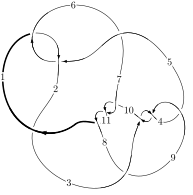
\includegraphics[width=112pt]{../../../GIT/diagram.site/Diagrams/png/392_11a_143.png}\\
\ \ \ A knot diagram\footnotemark}&
\allowdisplaybreaks
\textbf{Linearized knot diagam} \\
\cline{2-2}
 &
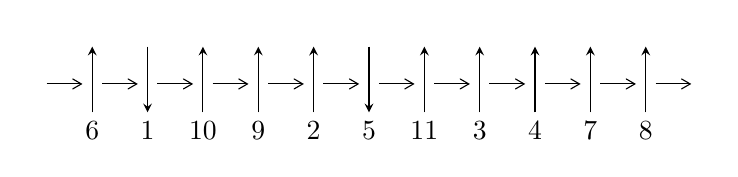
\begin{tikzpicture}[x=20pt, y=17pt]
	% nodes
	\node (C0) at (0, 0) {};
	\node (C1) at (1, 0) {};
	\node (C1U) at (1, +1) {};
	\node (C1D) at (1, -1) {6};

	\node (C2) at (2, 0) {};
	\node (C2U) at (2, +1) {};
	\node (C2D) at (2, -1) {1};

	\node (C3) at (3, 0) {};
	\node (C3U) at (3, +1) {};
	\node (C3D) at (3, -1) {10};

	\node (C4) at (4, 0) {};
	\node (C4U) at (4, +1) {};
	\node (C4D) at (4, -1) {9};

	\node (C5) at (5, 0) {};
	\node (C5U) at (5, +1) {};
	\node (C5D) at (5, -1) {2};

	\node (C6) at (6, 0) {};
	\node (C6U) at (6, +1) {};
	\node (C6D) at (6, -1) {5};

	\node (C7) at (7, 0) {};
	\node (C7U) at (7, +1) {};
	\node (C7D) at (7, -1) {11};

	\node (C8) at (8, 0) {};
	\node (C8U) at (8, +1) {};
	\node (C8D) at (8, -1) {3};

	\node (C9) at (9, 0) {};
	\node (C9U) at (9, +1) {};
	\node (C9D) at (9, -1) {4};

	\node (C10) at (10, 0) {};
	\node (C10U) at (10, +1) {};
	\node (C10D) at (10, -1) {7};

	\node (C11) at (11, 0) {};
	\node (C11U) at (11, +1) {};
	\node (C11D) at (11, -1) {8};
	\node (C12) at (12, 0) {};

	% arrows
	\draw[->,>={angle 60}]
	(C0) edge (C1) (C1) edge (C2) (C2) edge (C3) (C3) edge (C4) (C4) edge (C5) (C5) edge (C6) (C6) edge (C7) (C7) edge (C8) (C8) edge (C9) (C9) edge (C10) (C10) edge (C11) (C11) edge (C12) ;	\draw[->,>=stealth]
	(C1D) edge (C1U) (C2U) edge (C2D) (C3D) edge (C3U) (C4D) edge (C4U) (C5D) edge (C5U) (C6U) edge (C6D) (C7D) edge (C7U) (C8D) edge (C8U) (C9D) edge (C9U) (C10D) edge (C10U) (C11D) edge (C11U) ;
	\end{tikzpicture} \\
\hhline{~~} \\& 
\textbf{Solving Sequence} \\ \cline{2-2} 
 &
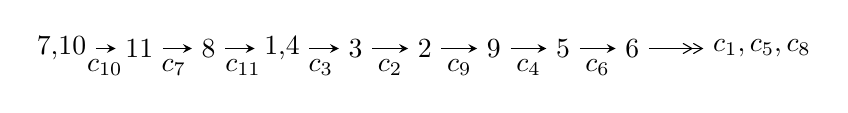
\begin{tikzpicture}[x=25pt, y=7pt]
	% node
	\node (A0) at (-1/8, 0) {7,10};
	\node (A1) at (1, 0) {11};
	\node (A2) at (2, 0) {8};
	\node (A3) at (49/16, 0) {1,4};
	\node (A4) at (33/8, 0) {3};
	\node (A5) at (41/8, 0) {2};
	\node (A6) at (49/8, 0) {9};
	\node (A7) at (57/8, 0) {5};
	\node (A8) at (65/8, 0) {6};
	\node (C1) at (1/2, -1) {$c_{10}$};
	\node (C2) at (3/2, -1) {$c_{7}$};
	\node (C3) at (5/2, -1) {$c_{11}$};
	\node (C4) at (29/8, -1) {$c_{3}$};
	\node (C5) at (37/8, -1) {$c_{2}$};
	\node (C6) at (45/8, -1) {$c_{9}$};
	\node (C7) at (53/8, -1) {$c_{4}$};
	\node (C8) at (61/8, -1) {$c_{6}$};
	\node (A9) at (10, 0) {$c_{1},c_{5},c_{8}$};

	% edge
	\draw[->,>=stealth]	
	(A0) edge (A1) (A1) edge (A2) (A2) edge (A3) (A3) edge (A4) (A4) edge (A5) (A5) edge (A6) (A6) edge (A7) (A7) edge (A8) ;
	\draw[->>,>={angle 60}]	
	(A8) edge (A9);
\end{tikzpicture} \\ 

\end{tabular} \\

\footnotetext{
The image of knot diagram is generated by the software ``\textbf{Draw programme}" developed by Andrew Bartholomew(\url{http://www.layer8.co.uk/maths/draw/index.htm\#Running-draw}), where we modified some parts for our purpose(\url{https://github.com/CATsTAILs/LinksPainter}).
}\phantom \\ \newline 
\centering \textbf{Ideals for irreducible components\footnotemark of $X_{\text{par}}$} 
 
\begin{align*}
I^u_{1}&=\langle 
3.31268\times10^{32} u^{49}-5.56961\times10^{32} u^{48}+\cdots+3.84136\times10^{32} b+1.21137\times10^{33},\\
\phantom{I^u_{1}}&\phantom{= \langle  }-1.01160\times10^{33} u^{49}-2.15416\times10^{33} u^{48}+\cdots+4.60963\times10^{33} a+6.11980\times10^{33},\\
\phantom{I^u_{1}}&\phantom{= \langle  }u^{50}-3 u^{49}+\cdots-14 u-3\rangle \\
I^u_{2}&=\langle 
-2 a^3+3 a^2+5 b-15 a+7,\;a^4-2 a^3+7 a^2-6 a+3,\;u+1\rangle \\
I^u_{3}&=\langle 
b,\;a^2- a+1,\;u-1\rangle \\
\\
\end{align*}
\raggedright * 3 irreducible components of $\dim_{\mathbb{C}}=0$, with total 56 representations.\\
\footnotetext{All coefficients of polynomials are rational numbers. But the coefficients are sometimes approximated in decimal forms when there is not enough margin.}
\newpage
\renewcommand{\arraystretch}{1}
\centering \section*{I. $I^u_{1}= \langle 3.31\times10^{32} u^{49}-5.57\times10^{32} u^{48}+\cdots+3.84\times10^{32} b+1.21\times10^{33},\;-1.01\times10^{33} u^{49}-2.15\times10^{33} u^{48}+\cdots+4.61\times10^{33} a+6.12\times10^{33},\;u^{50}-3 u^{49}+\cdots-14 u-3 \rangle$}
\flushleft \textbf{(i) Arc colorings}\\
\begin{tabular}{m{7pt} m{180pt} m{7pt} m{180pt} }
\flushright $a_{7}=$&$\begin{pmatrix}0\\u\end{pmatrix}$ \\
\flushright $a_{10}=$&$\begin{pmatrix}1\\0\end{pmatrix}$ \\
\flushright $a_{11}=$&$\begin{pmatrix}1\\- u^2\end{pmatrix}$ \\
\flushright $a_{8}=$&$\begin{pmatrix}u\\- u^3+u\end{pmatrix}$ \\
\flushright $a_{1}=$&$\begin{pmatrix}- u^2+1\\u^4-2 u^2\end{pmatrix}$ \\
\flushright $a_{4}=$&$\begin{pmatrix}0.219454 u^{49}+0.467318 u^{48}+\cdots+9.86130 u-1.32761\\-0.862372 u^{49}+1.44991 u^{48}+\cdots-16.7135 u-3.15351\end{pmatrix}$ \\
\flushright $a_{3}=$&$\begin{pmatrix}1.08183 u^{49}-0.982587 u^{48}+\cdots+26.5748 u+1.82589\\-0.862372 u^{49}+1.44991 u^{48}+\cdots-16.7135 u-3.15351\end{pmatrix}$ \\
\flushright $a_{2}=$&$\begin{pmatrix}0.247278 u^{49}+0.359922 u^{48}+\cdots+11.7803 u-0.445043\\-0.895841 u^{49}+1.30207 u^{48}+\cdots-19.0363 u-3.62861\end{pmatrix}$ \\
\flushright $a_{9}=$&$\begin{pmatrix}-0.694954 u^{49}+1.84791 u^{48}+\cdots+28.4151 u+4.77905\\0.141172 u^{49}-0.0191976 u^{48}+\cdots+5.14402 u-0.584566\end{pmatrix}$ \\
\flushright $a_{5}=$&$\begin{pmatrix}-0.562523 u^{49}+0.817800 u^{48}+\cdots-8.66416 u+1.58746\\0.649198 u^{49}-0.790264 u^{48}+\cdots+15.0431 u+2.83582\end{pmatrix}$ \\
\flushright $a_{6}=$&$\begin{pmatrix}-0.152066 u^{49}+0.970436 u^{48}+\cdots+28.0155 u+3.66927\\-0.384959 u^{49}+0.691554 u^{48}+\cdots-5.39208 u-2.02124\end{pmatrix}$\\ \flushright $a_{6}=$&$\begin{pmatrix}-0.152066 u^{49}+0.970436 u^{48}+\cdots+28.0155 u+3.66927\\-0.384959 u^{49}+0.691554 u^{48}+\cdots-5.39208 u-2.02124\end{pmatrix}$\\&\end{tabular}
\flushleft \textbf{(ii) Obstruction class $= -1$}\\~\\
\flushleft \textbf{(iii) Cusp Shapes $= -0.874649 u^{49}+2.02419 u^{48}+\cdots+4.43493 u+1.54316$}\\~\\
\newpage\renewcommand{\arraystretch}{1}
\flushleft \textbf{(iv) u-Polynomials at the component}\newline \\
\begin{tabular}{m{50pt}|m{274pt}}
Crossings & \hspace{64pt}u-Polynomials at each crossing \\
\hline $$\begin{aligned}c_{1},c_{5}\end{aligned}$$&$\begin{aligned}
&u^{50}-2 u^{49}+\cdots-3 u+3
\end{aligned}$\\
\hline $$\begin{aligned}c_{2},c_{6}\end{aligned}$$&$\begin{aligned}
&u^{50}+16 u^{49}+\cdots-39 u+9
\end{aligned}$\\
\hline $$\begin{aligned}c_{3},c_{4},c_{9}\end{aligned}$$&$\begin{aligned}
&u^{50}- u^{49}+\cdots+16 u-4
\end{aligned}$\\
\hline $$\begin{aligned}c_{7},c_{10},c_{11}\end{aligned}$$&$\begin{aligned}
&u^{50}-3 u^{49}+\cdots-14 u-3
\end{aligned}$\\
\hline $$\begin{aligned}c_{8}\end{aligned}$$&$\begin{aligned}
&u^{50}+u^{49}+\cdots+928 u-404
\end{aligned}$\\
\hline
\end{tabular}\\~\\
\newpage\renewcommand{\arraystretch}{1}
\flushleft \textbf{(v) Riley Polynomials at the component}\newline \\
\begin{tabular}{m{50pt}|m{274pt}}
Crossings & \hspace{64pt}Riley Polynomials at each crossing \\
\hline $$\begin{aligned}c_{1},c_{5}\end{aligned}$$&$\begin{aligned}
&y^{50}+16 y^{49}+\cdots-39 y+9
\end{aligned}$\\
\hline $$\begin{aligned}c_{2},c_{6}\end{aligned}$$&$\begin{aligned}
&y^{50}+40 y^{49}+\cdots-11439 y+81
\end{aligned}$\\
\hline $$\begin{aligned}c_{3},c_{4},c_{9}\end{aligned}$$&$\begin{aligned}
&y^{50}+45 y^{49}+\cdots-480 y^2+16
\end{aligned}$\\
\hline $$\begin{aligned}c_{7},c_{10},c_{11}\end{aligned}$$&$\begin{aligned}
&y^{50}-49 y^{49}+\cdots+68 y+9
\end{aligned}$\\
\hline $$\begin{aligned}c_{8}\end{aligned}$$&$\begin{aligned}
&y^{50}-15 y^{49}+\cdots+470400 y+163216
\end{aligned}$\\
\hline
\end{tabular}\\~\\
\newpage\flushleft \textbf{(vi) Complex Volumes and Cusp Shapes}
$$\begin{array}{c|c|c}  
\text{Solutions to }I^u_{1}& \I (\text{vol} + \sqrt{-1}CS) & \text{Cusp shape}\\
 \hline 
\begin{aligned}
u &= -0.768044 + 0.620254 I \\
a &= \phantom{-}0.51382 + 1.55754 I \\
b &= \phantom{-}0.223518 + 1.133800 I\end{aligned}
 & \phantom{-}0.52020 - 1.74042 I & \phantom{-}8.32117 + 2.63326 I \\ \hline\begin{aligned}
u &= -0.768044 - 0.620254 I \\
a &= \phantom{-}0.51382 - 1.55754 I \\
b &= \phantom{-}0.223518 - 1.133800 I\end{aligned}
 & \phantom{-}0.52020 + 1.74042 I & \phantom{-}8.32117 - 2.63326 I \\ \hline\begin{aligned}
u &= -0.357982 + 0.888739 I \\
a &= -0.66589 - 2.42275 I \\
b &= \phantom{-}0.310740 - 1.355660 I\end{aligned}
 & -1.38805 - 9.13876 I & \phantom{-}5.39526 + 7.47528 I \\ \hline\begin{aligned}
u &= -0.357982 - 0.888739 I \\
a &= -0.66589 + 2.42275 I \\
b &= \phantom{-}0.310740 + 1.355660 I\end{aligned}
 & -1.38805 + 9.13876 I & \phantom{-}5.39526 - 7.47528 I \\ \hline\begin{aligned}
u &= -0.419643 + 0.836664 I \\
a &= \phantom{-}0.70010 + 2.28634 I \\
b &= -0.299889 + 1.309250 I\end{aligned}
 & -0.58057 - 3.35428 I & \phantom{-}6.95050 + 2.72855 I \\ \hline\begin{aligned}
u &= -0.419643 - 0.836664 I \\
a &= \phantom{-}0.70010 - 2.28634 I \\
b &= -0.299889 - 1.309250 I\end{aligned}
 & -0.58057 + 3.35428 I & \phantom{-}6.95050 - 2.72855 I \\ \hline\begin{aligned}
u &= -0.875258 + 0.621898 I \\
a &= -0.48983 - 1.56500 I \\
b &= -0.261961 - 1.228410 I\end{aligned}
 & \phantom{-}0.20741 + 3.87448 I & \phantom{-}7.86992 - 3.23394 I \\ \hline\begin{aligned}
u &= -0.875258 - 0.621898 I \\
a &= -0.48983 + 1.56500 I \\
b &= -0.261961 + 1.228410 I\end{aligned}
 & \phantom{-}0.20741 - 3.87448 I & \phantom{-}7.86992 + 3.23394 I \\ \hline\begin{aligned}
u &= \phantom{-}0.600873 + 0.702881 I \\
a &= -0.263588 - 0.464164 I \\
b &= -0.718050 - 0.066541 I\end{aligned}
 & \phantom{-}3.72925 - 0.33634 I & \phantom{-}12.06779 - 0.57902 I \\ \hline\begin{aligned}
u &= \phantom{-}0.600873 - 0.702881 I \\
a &= -0.263588 + 0.464164 I \\
b &= -0.718050 + 0.066541 I\end{aligned}
 & \phantom{-}3.72925 + 0.33634 I & \phantom{-}12.06779 + 0.57902 I\\
 \hline 
 \end{array}$$\newpage$$\begin{array}{c|c|c}  
\text{Solutions to }I^u_{1}& \I (\text{vol} + \sqrt{-1}CS) & \text{Cusp shape}\\
 \hline 
\begin{aligned}
u &= \phantom{-}0.494891 + 0.774626 I \\
a &= \phantom{-}0.302543 + 0.581565 I \\
b &= \phantom{-}0.737047 + 0.149487 I\end{aligned}
 & \phantom{-}3.36565 + 5.33408 I & \phantom{-}10.62323 - 6.45202 I \\ \hline\begin{aligned}
u &= \phantom{-}0.494891 - 0.774626 I \\
a &= \phantom{-}0.302543 - 0.581565 I \\
b &= \phantom{-}0.737047 - 0.149487 I\end{aligned}
 & \phantom{-}3.36565 - 5.33408 I & \phantom{-}10.62323 + 6.45202 I \\ \hline\begin{aligned}
u &= -1.065360 + 0.257655 I \\
a &= -0.23062 - 1.52209 I \\
b &= -0.10488 - 1.42170 I\end{aligned}
 & -4.48476 + 0.36744 I & \phantom{-}2.34065 + 0.74088 I \\ \hline\begin{aligned}
u &= -1.065360 - 0.257655 I \\
a &= -0.23062 + 1.52209 I \\
b &= -0.10488 + 1.42170 I\end{aligned}
 & -4.48476 - 0.36744 I & \phantom{-}2.34065 - 0.74088 I \\ \hline\begin{aligned}
u &= \phantom{-}1.100360 + 0.172393 I \\
a &= -0.0409123 + 0.0182444 I \\
b &= -0.313724 + 0.372597 I\end{aligned}
 & \phantom{-}1.27025 + 1.19184 I & \phantom{-}7.00000 + 2.50368 I \\ \hline\begin{aligned}
u &= \phantom{-}1.100360 - 0.172393 I \\
a &= -0.0409123 - 0.0182444 I \\
b &= -0.313724 - 0.372597 I\end{aligned}
 & \phantom{-}1.27025 - 1.19184 I & \phantom{-}7.00000 - 2.50368 I \\ \hline\begin{aligned}
u &= -0.207647 + 0.672129 I \\
a &= -1.26448 - 2.57161 I \\
b &= \phantom{-}0.182493 - 1.383300 I\end{aligned}
 & -6.96148 - 3.84491 I & -1.20333 + 4.74598 I \\ \hline\begin{aligned}
u &= -0.207647 - 0.672129 I \\
a &= -1.26448 + 2.57161 I \\
b &= \phantom{-}0.182493 + 1.383300 I\end{aligned}
 & -6.96148 + 3.84491 I & -1.20333 - 4.74598 I \\ \hline\begin{aligned}
u &= -1.349830 + 0.119644 I \\
a &= \phantom{-}0.951187 + 0.404966 I \\
b &= -0.680112 + 0.135570 I\end{aligned}
 & \phantom{-}2.86347 - 3.60406 I & \phantom{-0.000000 } 0 \\ \hline\begin{aligned}
u &= -1.349830 - 0.119644 I \\
a &= \phantom{-}0.951187 - 0.404966 I \\
b &= -0.680112 - 0.135570 I\end{aligned}
 & \phantom{-}2.86347 + 3.60406 I & \phantom{-0.000000 } 0\\
 \hline 
 \end{array}$$\newpage$$\begin{array}{c|c|c}  
\text{Solutions to }I^u_{1}& \I (\text{vol} + \sqrt{-1}CS) & \text{Cusp shape}\\
 \hline 
\begin{aligned}
u &= -0.419371 + 0.489432 I \\
a &= \phantom{-}1.23676 + 1.66984 I \\
b &= -0.103698 + 1.289300 I\end{aligned}
 & -3.33666 - 1.69681 I & \phantom{-}6.02735 + 3.86873 I \\ \hline\begin{aligned}
u &= -0.419371 - 0.489432 I \\
a &= \phantom{-}1.23676 - 1.66984 I \\
b &= -0.103698 - 1.289300 I\end{aligned}
 & -3.33666 + 1.69681 I & \phantom{-}6.02735 - 3.86873 I \\ \hline\begin{aligned}
u &= \phantom{-}1.352170 + 0.098819 I \\
a &= \phantom{-}1.161170 + 0.144436 I \\
b &= -0.211969 - 1.214280 I\end{aligned}
 & -0.313966 - 0.436878 I & \phantom{-0.000000 } 0 \\ \hline\begin{aligned}
u &= \phantom{-}1.352170 - 0.098819 I \\
a &= \phantom{-}1.161170 - 0.144436 I \\
b &= -0.211969 + 1.214280 I\end{aligned}
 & -0.313966 + 0.436878 I & \phantom{-0.000000 } 0 \\ \hline\begin{aligned}
u &= -1.356110 + 0.045936 I \\
a &= -0.03253 - 1.71582 I \\
b &= -0.02262 - 1.56889 I\end{aligned}
 & -0.83159 - 2.75739 I & \phantom{-0.000000 } 0 \\ \hline\begin{aligned}
u &= -1.356110 - 0.045936 I \\
a &= -0.03253 + 1.71582 I \\
b &= -0.02262 + 1.56889 I\end{aligned}
 & -0.83159 + 2.75739 I & \phantom{-0.000000 } 0 \\ \hline\begin{aligned}
u &= \phantom{-}1.391060 + 0.243928 I \\
a &= \phantom{-}1.57875 - 0.80925 I \\
b &= -0.287890 - 1.351540 I\end{aligned}
 & -1.84682 + 7.14521 I & \phantom{-0.000000 } 0 \\ \hline\begin{aligned}
u &= \phantom{-}1.391060 - 0.243928 I \\
a &= \phantom{-}1.57875 + 0.80925 I \\
b &= -0.287890 + 1.351540 I\end{aligned}
 & -1.84682 - 7.14521 I & \phantom{-0.000000 } 0 \\ \hline\begin{aligned}
u &= -1.43839\phantom{ +0.000000I} \\
a &= -0.748101\phantom{ +0.000000I} \\
b &= \phantom{-}0.770058\phantom{ +0.000000I}\end{aligned}
 & \phantom{-}6.46721\phantom{ +0.000000I} & \phantom{-0.000000 } 0 \\ \hline\begin{aligned}
u &= \phantom{-}1.43734 + 0.14823 I \\
a &= -1.093440 + 0.493494 I \\
b &= \phantom{-}0.323552 + 1.255700 I\end{aligned}
 & \phantom{-}2.58460 + 3.94905 I & \phantom{-0.000000 } 0\\
 \hline 
 \end{array}$$\newpage$$\begin{array}{c|c|c}  
\text{Solutions to }I^u_{1}& \I (\text{vol} + \sqrt{-1}CS) & \text{Cusp shape}\\
 \hline 
\begin{aligned}
u &= \phantom{-}1.43734 - 0.14823 I \\
a &= -1.093440 - 0.493494 I \\
b &= \phantom{-}0.323552 - 1.255700 I\end{aligned}
 & \phantom{-}2.58460 - 3.94905 I & \phantom{-0.000000 } 0 \\ \hline\begin{aligned}
u &= -0.513376 + 0.156185 I \\
a &= \phantom{-}0.12350 + 1.97974 I \\
b &= \phantom{-}0.024574 + 0.485591 I\end{aligned}
 & \phantom{-}0.74464 - 2.36364 I & \phantom{-}3.62478 + 4.11961 I \\ \hline\begin{aligned}
u &= -0.513376 - 0.156185 I \\
a &= \phantom{-}0.12350 - 1.97974 I \\
b &= \phantom{-}0.024574 - 0.485591 I\end{aligned}
 & \phantom{-}0.74464 + 2.36364 I & \phantom{-}3.62478 - 4.11961 I \\ \hline\begin{aligned}
u &= \phantom{-}0.099189 + 0.524649 I \\
a &= -0.042705 + 1.015670 I \\
b &= \phantom{-}0.469409 + 0.309538 I\end{aligned}
 & -1.63114 + 1.42356 I & \phantom{-}2.31879 - 5.63109 I \\ \hline\begin{aligned}
u &= \phantom{-}0.099189 - 0.524649 I \\
a &= -0.042705 - 1.015670 I \\
b &= \phantom{-}0.469409 - 0.309538 I\end{aligned}
 & -1.63114 - 1.42356 I & \phantom{-}2.31879 + 5.63109 I \\ \hline\begin{aligned}
u &= \phantom{-}1.48543 + 0.34428 I \\
a &= \phantom{-}1.24716 - 1.34114 I \\
b &= -0.36507 - 1.42866 I\end{aligned}
 & \phantom{-}4.5437 + 13.6084 I & \phantom{-0.000000 } 0 \\ \hline\begin{aligned}
u &= \phantom{-}1.48543 - 0.34428 I \\
a &= \phantom{-}1.24716 + 1.34114 I \\
b &= -0.36507 + 1.42866 I\end{aligned}
 & \phantom{-}4.5437 - 13.6084 I & \phantom{-0.000000 } 0 \\ \hline\begin{aligned}
u &= \phantom{-}1.51636 + 0.16091 I \\
a &= \phantom{-}0.098166 + 0.420372 I \\
b &= -0.558023 + 0.923611 I\end{aligned}
 & \phantom{-}7.88001 + 4.14120 I & \phantom{-0.000000 } 0 \\ \hline\begin{aligned}
u &= \phantom{-}1.51636 - 0.16091 I \\
a &= \phantom{-}0.098166 - 0.420372 I \\
b &= -0.558023 - 0.923611 I\end{aligned}
 & \phantom{-}7.88001 - 4.14120 I & \phantom{-0.000000 } 0 \\ \hline\begin{aligned}
u &= \phantom{-}1.50169 + 0.30522 I \\
a &= -1.16719 + 1.21068 I \\
b &= \phantom{-}0.37957 + 1.39957 I\end{aligned}
 & \phantom{-}5.64838 + 7.50037 I & \phantom{-0.000000 } 0\\
 \hline 
 \end{array}$$\newpage$$\begin{array}{c|c|c}  
\text{Solutions to }I^u_{1}& \I (\text{vol} + \sqrt{-1}CS) & \text{Cusp shape}\\
 \hline 
\begin{aligned}
u &= \phantom{-}1.50169 - 0.30522 I \\
a &= -1.16719 - 1.21068 I \\
b &= \phantom{-}0.37957 - 1.39957 I\end{aligned}
 & \phantom{-}5.64838 - 7.50037 I & \phantom{-0.000000 } 0 \\ \hline\begin{aligned}
u &= \phantom{-}1.53335 + 0.09779 I \\
a &= -0.209409 - 0.465882 I \\
b &= \phantom{-}0.526883 - 0.998341 I\end{aligned}
 & \phantom{-}8.31731 - 1.99153 I & \phantom{-0.000000 } 0 \\ \hline\begin{aligned}
u &= \phantom{-}1.53335 - 0.09779 I \\
a &= -0.209409 + 0.465882 I \\
b &= \phantom{-}0.526883 + 0.998341 I\end{aligned}
 & \phantom{-}8.31731 + 1.99153 I & \phantom{-0.000000 } 0 \\ \hline\begin{aligned}
u &= -1.51832 + 0.26912 I \\
a &= \phantom{-}0.407229 + 0.580854 I \\
b &= -0.874042 + 0.265626 I\end{aligned}
 & \phantom{-}9.92580 - 9.13602 I & \phantom{-0.000000 } 0 \\ \hline\begin{aligned}
u &= -1.51832 - 0.26912 I \\
a &= \phantom{-}0.407229 - 0.580854 I \\
b &= -0.874042 - 0.265626 I\end{aligned}
 & \phantom{-}9.92580 + 9.13602 I & \phantom{-0.000000 } 0 \\ \hline\begin{aligned}
u &= -1.53487 + 0.21619 I \\
a &= -0.418285 - 0.467881 I \\
b &= \phantom{-}0.882710 - 0.212600 I\end{aligned}
 & \phantom{-}10.74210 - 2.95976 I & \phantom{-0.000000 } 0 \\ \hline\begin{aligned}
u &= -1.53487 - 0.21619 I \\
a &= -0.418285 + 0.467881 I \\
b &= \phantom{-}0.882710 + 0.212600 I\end{aligned}
 & \phantom{-}10.74210 + 2.95976 I & \phantom{-0.000000 } 0 \\ \hline\begin{aligned}
u &= \phantom{-}0.377548\phantom{ +0.000000I} \\
a &= \phantom{-}0.538429\phantom{ +0.000000I} \\
b &= -0.387989\phantom{ +0.000000I}\end{aligned}
 & \phantom{-}0.630546\phantom{ +0.000000I} & \phantom{-}15.8700\phantom{ +0.000000I} \\ \hline\begin{aligned}
u &= -0.096486 + 0.258092 I \\
a &= -4.46333 - 1.70481 I \\
b &= \phantom{-}0.050400 - 1.397800 I\end{aligned}
 & -5.03824 + 1.88230 I & -0.03756 - 2.83434 I \\ \hline\begin{aligned}
u &= -0.096486 - 0.258092 I \\
a &= -4.46333 + 1.70481 I \\
b &= \phantom{-}0.050400 + 1.397800 I\end{aligned}
 & -5.03824 - 1.88230 I & -0.03756 + 2.83434 I\\
 \hline 
 \end{array}$$\newpage\newpage\renewcommand{\arraystretch}{1}
\centering \section*{II. $I^u_{2}= \langle -2 a^3+3 a^2+5 b-15 a+7,\;a^4-2 a^3+7 a^2-6 a+3,\;u+1 \rangle$}
\flushleft \textbf{(i) Arc colorings}\\
\begin{tabular}{m{7pt} m{180pt} m{7pt} m{180pt} }
\flushright $a_{7}=$&$\begin{pmatrix}0\\-1\end{pmatrix}$ \\
\flushright $a_{10}=$&$\begin{pmatrix}1\\0\end{pmatrix}$ \\
\flushright $a_{11}=$&$\begin{pmatrix}1\\-1\end{pmatrix}$ \\
\flushright $a_{8}=$&$\begin{pmatrix}-1\\0\end{pmatrix}$ \\
\flushright $a_{1}=$&$\begin{pmatrix}0\\-1\end{pmatrix}$ \\
\flushright $a_{4}=$&$\begin{pmatrix}a\\\frac{2}{5} a^3-\frac{3}{5} a^2+3 a-\frac{7}{5}\end{pmatrix}$ \\
\flushright $a_{3}=$&$\begin{pmatrix}-\frac{2}{5} a^3+\frac{3}{5} a^2-2 a+\frac{7}{5}\\\frac{2}{5} a^3-\frac{3}{5} a^2+3 a-\frac{7}{5}\end{pmatrix}$ \\
\flushright $a_{2}=$&$\begin{pmatrix}-\frac{2}{5} a^3+\frac{3}{5} a^2-2 a+\frac{7}{5}\\\frac{4}{5} a^3-\frac{6}{5} a^2+5 a-\frac{14}{5}\end{pmatrix}$ \\
\flushright $a_{9}=$&$\begin{pmatrix}\frac{1}{5} a^3+\frac{1}{5} a^2+a-\frac{1}{5}\\-2\end{pmatrix}$ \\
\flushright $a_{5}=$&$\begin{pmatrix}\frac{2}{5} a^3-\frac{3}{5} a^2+2 a-\frac{7}{5}\\-\frac{2}{5} a^3+\frac{3}{5} a^2-3 a+\frac{7}{5}\end{pmatrix}$ \\
\flushright $a_{6}=$&$\begin{pmatrix}\frac{2}{5} a^3-\frac{3}{5} a^2+2 a-\frac{2}{5}\\-\frac{1}{5} a^3-\frac{1}{5} a^2- a-\frac{9}{5}\end{pmatrix}$\\ \flushright $a_{6}=$&$\begin{pmatrix}\frac{2}{5} a^3-\frac{3}{5} a^2+2 a-\frac{2}{5}\\-\frac{1}{5} a^3-\frac{1}{5} a^2- a-\frac{9}{5}\end{pmatrix}$\\&\end{tabular}
\flushleft \textbf{(ii) Obstruction class $= 1$}\\~\\
\flushleft \textbf{(iii) Cusp Shapes $= -\frac{8}{5} a^3+\frac{12}{5} a^2-8 a+\frac{48}{5}$}\\~\\
\newpage\renewcommand{\arraystretch}{1}
\flushleft \textbf{(iv) u-Polynomials at the component}\newline \\
\begin{tabular}{m{50pt}|m{274pt}}
Crossings & \hspace{64pt}u-Polynomials at each crossing \\
\hline $$\begin{aligned}c_{1}\end{aligned}$$&$\begin{aligned}
&(u^2- u+1)^2
\end{aligned}$\\
\hline $$\begin{aligned}c_{2},c_{5},c_{6}\end{aligned}$$&$\begin{aligned}
&(u^2+u+1)^2
\end{aligned}$\\
\hline $$\begin{aligned}c_{3},c_{4},c_{8}\\c_{9}\end{aligned}$$&$\begin{aligned}
&(u^2+2)^2
\end{aligned}$\\
\hline $$\begin{aligned}c_{7}\end{aligned}$$&$\begin{aligned}
&(u-1)^4
\end{aligned}$\\
\hline $$\begin{aligned}c_{10},c_{11}\end{aligned}$$&$\begin{aligned}
&(u+1)^4
\end{aligned}$\\
\hline
\end{tabular}\\~\\
\newpage\renewcommand{\arraystretch}{1}
\flushleft \textbf{(v) Riley Polynomials at the component}\newline \\
\begin{tabular}{m{50pt}|m{274pt}}
Crossings & \hspace{64pt}Riley Polynomials at each crossing \\
\hline $$\begin{aligned}c_{1},c_{2},c_{5}\\c_{6}\end{aligned}$$&$\begin{aligned}
&(y^2+y+1)^2
\end{aligned}$\\
\hline $$\begin{aligned}c_{3},c_{4},c_{8}\\c_{9}\end{aligned}$$&$\begin{aligned}
&(y+2)^4
\end{aligned}$\\
\hline $$\begin{aligned}c_{7},c_{10},c_{11}\end{aligned}$$&$\begin{aligned}
&(y-1)^4
\end{aligned}$\\
\hline
\end{tabular}\\~\\
\newpage\flushleft \textbf{(vi) Complex Volumes and Cusp Shapes}
$$\begin{array}{c|c|c}  
\text{Solutions to }I^u_{2}& \I (\text{vol} + \sqrt{-1}CS) & \text{Cusp shape}\\
 \hline 
\begin{aligned}
u &= -1.00000\phantom{ +0.000000I} \\
a &= \phantom{-}0.500000 + 0.548188 I \\
b &= \phantom{-0.000000 -}1.414210 I\end{aligned}
 & -3.28987 + 2.02988 I & \phantom{-}6.00000 - 3.46410 I \\ \hline\begin{aligned}
u &= -1.00000\phantom{ +0.000000I} \\
a &= \phantom{-}0.500000 - 0.548188 I \\
b &= \phantom{-0.000000 } -1.414210 I\end{aligned}
 & -3.28987 - 2.02988 I & \phantom{-}6.00000 + 3.46410 I \\ \hline\begin{aligned}
u &= -1.00000\phantom{ +0.000000I} \\
a &= \phantom{-}0.50000 + 2.28024 I \\
b &= \phantom{-0.000000 -}1.414210 I\end{aligned}
 & -3.28987 - 2.02988 I & \phantom{-}6.00000 + 3.46410 I \\ \hline\begin{aligned}
u &= -1.00000\phantom{ +0.000000I} \\
a &= \phantom{-}0.50000 - 2.28024 I \\
b &= \phantom{-0.000000 } -1.414210 I\end{aligned}
 & -3.28987 + 2.02988 I & \phantom{-}6.00000 - 3.46410 I\\
 \hline 
 \end{array}$$\newpage\newpage\renewcommand{\arraystretch}{1}
\centering \section*{III. $I^u_{3}= \langle b,\;a^2- a+1,\;u-1 \rangle$}
\flushleft \textbf{(i) Arc colorings}\\
\begin{tabular}{m{7pt} m{180pt} m{7pt} m{180pt} }
\flushright $a_{7}=$&$\begin{pmatrix}0\\1\end{pmatrix}$ \\
\flushright $a_{10}=$&$\begin{pmatrix}1\\0\end{pmatrix}$ \\
\flushright $a_{11}=$&$\begin{pmatrix}1\\-1\end{pmatrix}$ \\
\flushright $a_{8}=$&$\begin{pmatrix}1\\0\end{pmatrix}$ \\
\flushright $a_{1}=$&$\begin{pmatrix}0\\-1\end{pmatrix}$ \\
\flushright $a_{4}=$&$\begin{pmatrix}a\\0\end{pmatrix}$ \\
\flushright $a_{3}=$&$\begin{pmatrix}a\\0\end{pmatrix}$ \\
\flushright $a_{2}=$&$\begin{pmatrix}a\\- a\end{pmatrix}$ \\
\flushright $a_{9}=$&$\begin{pmatrix}1\\0\end{pmatrix}$ \\
\flushright $a_{5}=$&$\begin{pmatrix}a\\0\end{pmatrix}$ \\
\flushright $a_{6}=$&$\begin{pmatrix}a-1\\1\end{pmatrix}$\\ \flushright $a_{6}=$&$\begin{pmatrix}a-1\\1\end{pmatrix}$\\&\end{tabular}
\flushleft \textbf{(ii) Obstruction class $= 1$}\\~\\
\flushleft \textbf{(iii) Cusp Shapes $= 4 a+10$}\\~\\
\newpage\renewcommand{\arraystretch}{1}
\flushleft \textbf{(iv) u-Polynomials at the component}\newline \\
\begin{tabular}{m{50pt}|m{274pt}}
Crossings & \hspace{64pt}u-Polynomials at each crossing \\
\hline $$\begin{aligned}c_{1},c_{2},c_{6}\end{aligned}$$&$\begin{aligned}
&u^2+u+1
\end{aligned}$\\
\hline $$\begin{aligned}c_{3},c_{4},c_{8}\\c_{9}\end{aligned}$$&$\begin{aligned}
&u^2
\end{aligned}$\\
\hline $$\begin{aligned}c_{5}\end{aligned}$$&$\begin{aligned}
&u^2- u+1
\end{aligned}$\\
\hline $$\begin{aligned}c_{7}\end{aligned}$$&$\begin{aligned}
&(u+1)^2
\end{aligned}$\\
\hline $$\begin{aligned}c_{10},c_{11}\end{aligned}$$&$\begin{aligned}
&(u-1)^2
\end{aligned}$\\
\hline
\end{tabular}\\~\\
\newpage\renewcommand{\arraystretch}{1}
\flushleft \textbf{(v) Riley Polynomials at the component}\newline \\
\begin{tabular}{m{50pt}|m{274pt}}
Crossings & \hspace{64pt}Riley Polynomials at each crossing \\
\hline $$\begin{aligned}c_{1},c_{2},c_{5}\\c_{6}\end{aligned}$$&$\begin{aligned}
&y^2+y+1
\end{aligned}$\\
\hline $$\begin{aligned}c_{3},c_{4},c_{8}\\c_{9}\end{aligned}$$&$\begin{aligned}
&y^2
\end{aligned}$\\
\hline $$\begin{aligned}c_{7},c_{10},c_{11}\end{aligned}$$&$\begin{aligned}
&(y-1)^2
\end{aligned}$\\
\hline
\end{tabular}\\~\\
\newpage\flushleft \textbf{(vi) Complex Volumes and Cusp Shapes}
$$\begin{array}{c|c|c}  
\text{Solutions to }I^u_{3}& \I (\text{vol} + \sqrt{-1}CS) & \text{Cusp shape}\\
 \hline 
\begin{aligned}
u &= \phantom{-}1.00000\phantom{ +0.000000I} \\
a &= \phantom{-}0.500000 + 0.866025 I \\
b &= \phantom{-0.000000 } 0\end{aligned}
 & \phantom{-}1.64493 - 2.02988 I & \phantom{-}12.00000 + 3.46410 I \\ \hline\begin{aligned}
u &= \phantom{-}1.00000\phantom{ +0.000000I} \\
a &= \phantom{-}0.500000 - 0.866025 I \\
b &= \phantom{-0.000000 } 0\end{aligned}
 & \phantom{-}1.64493 + 2.02988 I & \phantom{-}12.00000 - 3.46410 I\\
 \hline 
 \end{array}$$\newpage
\newpage\renewcommand{\arraystretch}{1}
\centering \section*{ IV. u-Polynomials}
\begin{tabular}{m{50pt}|m{274pt}}
Crossings & \hspace{64pt}u-Polynomials at each crossing \\
\hline $$\begin{aligned}c_{1}\end{aligned}$$&$\begin{aligned}
&((u^2- u+1)^2)(u^2+u+1)(u^{50}-2 u^{49}+\cdots-3 u+3)
\end{aligned}$\\
\hline $$\begin{aligned}c_{2},c_{6}\end{aligned}$$&$\begin{aligned}
&((u^2+u+1)^3)(u^{50}+16 u^{49}+\cdots-39 u+9)
\end{aligned}$\\
\hline $$\begin{aligned}c_{3},c_{4},c_{9}\end{aligned}$$&$\begin{aligned}
&u^2(u^2+2)^2(u^{50}- u^{49}+\cdots+16 u-4)
\end{aligned}$\\
\hline $$\begin{aligned}c_{5}\end{aligned}$$&$\begin{aligned}
&(u^2- u+1)(u^2+u+1)^2(u^{50}-2 u^{49}+\cdots-3 u+3)
\end{aligned}$\\
\hline $$\begin{aligned}c_{7}\end{aligned}$$&$\begin{aligned}
&((u-1)^4)(u+1)^2(u^{50}-3 u^{49}+\cdots-14 u-3)
\end{aligned}$\\
\hline $$\begin{aligned}c_{8}\end{aligned}$$&$\begin{aligned}
&u^2(u^2+2)^2(u^{50}+u^{49}+\cdots+928 u-404)
\end{aligned}$\\
\hline $$\begin{aligned}c_{10},c_{11}\end{aligned}$$&$\begin{aligned}
&((u-1)^2)(u+1)^4(u^{50}-3 u^{49}+\cdots-14 u-3)
\end{aligned}$\\
\hline
\end{tabular}\newpage\renewcommand{\arraystretch}{1}
\centering \section*{ V. Riley Polynomials}
\begin{tabular}{m{50pt}|m{274pt}}
Crossings & \hspace{64pt}Riley Polynomials at each crossing \\
\hline $$\begin{aligned}c_{1},c_{5}\end{aligned}$$&$\begin{aligned}
&((y^2+y+1)^3)(y^{50}+16 y^{49}+\cdots-39 y+9)
\end{aligned}$\\
\hline $$\begin{aligned}c_{2},c_{6}\end{aligned}$$&$\begin{aligned}
&((y^2+y+1)^3)(y^{50}+40 y^{49}+\cdots-11439 y+81)
\end{aligned}$\\
\hline $$\begin{aligned}c_{3},c_{4},c_{9}\end{aligned}$$&$\begin{aligned}
&y^2(y+2)^4(y^{50}+45 y^{49}+\cdots-480 y^{2}+16)
\end{aligned}$\\
\hline $$\begin{aligned}c_{7},c_{10},c_{11}\end{aligned}$$&$\begin{aligned}
&((y-1)^6)(y^{50}-49 y^{49}+\cdots+68 y+9)
\end{aligned}$\\
\hline $$\begin{aligned}c_{8}\end{aligned}$$&$\begin{aligned}
&y^2(y+2)^4(y^{50}-15 y^{49}+\cdots+470400 y+163216)
\end{aligned}$\\
\hline
\end{tabular}
\vskip 2pc
\end{document}